%%%%%%%%%%%%%%%%%%%%%%%%%%%%%%%%%%%%%%%%%
% Stylish Article
% LaTeX Template
% Version 2.2 (2020-10-22)
%
% This template has been downloaded from:
% http://www.LaTeXTemplates.com
%
% Original author:
% Mathias Legrand (legrand.mathias@gmail.com) 
% With extensive modifications by:
% Vel (vel@latextemplates.com)
%
% License:
% CC BY-NC-SA 3.0 (http://creativecommons.org/licenses/by-nc-sa/3.0/)
%
%%%%%%%%%%%%%%%%%%%%%%%%%%%%%%%%%%%%%%%%%

%----------------------------------------------------------------------------------------
%	PACKAGES AND OTHER DOCUMENT CONFIGURATIONS
%----------------------------------------------------------------------------------------

\documentclass[fleqn,10pt]{SelfArx} % Document font size and equations flushed left

\usepackage[fontset=none]{ctex}
\setCJKmainfont{Noto Serif CJK SC}
\setCJKsansfont{Noto Serif CJK SC}
\setCJKmonofont{Noto Sans CJK SC}

%----------------------------------------------------------------------------------------
%	COLUMNS
%----------------------------------------------------------------------------------------

\setlength{\columnsep}{0.55cm} % Distance between the two columns of text
\setlength{\fboxrule}{0.75pt} % Width of the border around the abstract

%----------------------------------------------------------------------------------------
%	COLORS
%----------------------------------------------------------------------------------------

\definecolor{color1}{RGB}{0,0,90} % Color of the article title and sections
\definecolor{color2}{RGB}{0,20,20} % Color of the boxes behind the abstract and headings

%----------------------------------------------------------------------------------------
%	HYPERLINKS
%----------------------------------------------------------------------------------------

\usepackage{hyperref} % Required for hyperlinks

\hypersetup{
	hidelinks,
	colorlinks,
	breaklinks=true,
	urlcolor=color2,
	citecolor=color1,
	linkcolor=color1,
	bookmarksopen=false,
	pdftitle={Title},
	pdfauthor={Author},
}

%----------------------------------------------------------------------------------------
%	ARTICLE INFORMATION
%----------------------------------------------------------------------------------------

\JournalInfo{基础物理学实验A3} % Journal information
\Archive{} % Additional notes (e.g. copyright, DOI, review/research article)

\PaperTitle{实验报告} % Article title

\Authors{} % Authors
\affiliation{} % Author affiliation

\Keywords{} % Keywords - if you don't want any simply remove all the text between the curly brackets
\newcommand{\keywordname}{Keywords} % Defines the keywords heading name

%----------------------------------------------------------------------------------------
%	ABSTRACT
%----------------------------------------------------------------------------------------

\Abstract{本实验利用激光衍射的方式,测量了不同种类的晶体的性质。既测量了一维晶体的衍射,还测量了二维晶体的晶格矢量。最后,我们利用傅里叶变换的方式测定了二维晶体的具体结构。}

%----------------------------------------------------------------------------------------

\begin{document}

\maketitle % Output the title and abstract box

\tableofcontents % Output the contents section

\thispagestyle{empty} % Removes page numbering from the first page

%----------------------------------------------------------------------------------------
%	ARTICLE CONTENTS
%----------------------------------------------------------------------------------------

\section{一维晶体光栅衍射的测量} % The \section*{} command stops section numbering

我们规定$q$为散射矢量($k_s-k_a$),设光栅常数为$a$,晶胞参量(也就是狭缝宽度)为$b$,利用衍射的基本知识,可以推出:$I=\frac{I_0}{N^2}(\frac{\sin{Nqa/2}}{\sin{(qa/2)}})^2(\frac{\sin{qb/2}}{qb/2})^2$。可以看出,对于一级散射矢量$q_1$,有$q_1a/2=\pi$,即$q_1a=2\pi$,已知$q_1$即可求出$a$。为了求$q_1$,设在第$N$个极大的时候,距离为$s_N$,此时,由衍射的知识可知:$q_1=\frac{2\pi}{\lambda}\frac{s_N}{NL}$,带回,$a=\frac{NL\lambda}{s_N}$

我们用激光打到待测一维样品上,可以观察到明显的衍射现象。测量结果如表\ref{tab:1}。
\begin{table}[htbp]
\centering
\begin{tabular}{|l|l|l|l|l|l|}
\hline
      & DG1  & DG2  & DG3 & DG4  & DG5  \\ \hline
N     & 5    & 10   & 12  & 10   & 11   \\ \hline
$s_N$ & 8.65 & 6.95 & 5.2 & 4.35 & 4.75 \\ \hline
\end{tabular}
\caption{一维晶体的衍射}
\label{tab:1}
\end{table}

实验的激光波长为$650nm$,保持间距$53.3cm$。根据前面的原理计算,可得到表\ref{tab:2}
\begin{table}[htbp]
\centering
\begin{tabular}{|l|l|l|l|l|l|}
\hline
\multicolumn{1}{|c|}{\textbf{}} &
  \multicolumn{1}{c|}{\textbf{DG1}} &
  \multicolumn{1}{c|}{\textbf{DG2}} &
  \multicolumn{1}{c|}{\textbf{DG3}} &
  \multicolumn{1}{c|}{\textbf{DG4}} &
  \multicolumn{1}{c|}{\textbf{DG5}} \\ \hline
q\_1($\mu m^{-1}$) &
  0.325 &
  0.126 &
  0.0786 &
  0.0789 &
  0.0783 \\ \hline
a($\mu m$) &
  19.35 &
  49.85 &
  79.95 &
  79.64 &
  80.23 \\ \hline
\end{tabular}
\caption{一维晶体的结构数据}
\label{tab:2}
\end{table}
%------------------------------------------------

\section{二维晶体的晶格矢量}

用上个部分的方法,我们同样可以计算出二维晶体的晶格矢量。

首先对于UC1到UC4,我们需要确定晶体周期。上部分给出了一个测量晶体结构大小参数的方法。为了测出周期,我们需要测量衍射图像在距离上重复的周期。(对于UC1到UC4而言,其为正方形的晶体结构,无论从哪个方向计算都可以得到所需要的结果,这里我们选择矩形晶体结构的任意一条边)测量用的激光和屏幕位置与第一部分相比不变。测量与计算得到的结果如表\ref{tab:3}。
\begin{table}[htbp]
\centering
\begin{tabular}{|l|l|l|l|l|}
\hline
\multicolumn{1}{|c|}{\textbf{}} &
  \multicolumn{1}{c|}{\textbf{UC1}} &
  \multicolumn{1}{c|}{\textbf{UC2}} &
  \multicolumn{1}{c|}{\textbf{UC3}} &
  \multicolumn{1}{c|}{\textbf{UC4}} \\ \hline
$N$        & 4    & 2    & 4    & 4    \\ \hline
$s_N(cm)$  & 4.65 & 3.45 & 6.9  & 4.7  \\ \hline
$a(\mu m)$ & 29.8 & 20.8 & 20.8 & 29.5 \\ \hline
\end{tabular}
\caption{二维晶体的晶体周期}
\label{tab:3}
\end{table}
接下来,需要判断晶体对应关系。首先,考虑到晶体D的交错结构,会使得$h+k=n_{odd}$(奇数)的那一级缺级,故UC3对应D。A与B的结构类似,但是由于A有着更小的晶体周期,其散射光斑的缺级应该在N更小的部分出现,故而缺级在$N=2$出现的UC2是A。最后考虑1和4,目测可知1有更强的中心亮度,故而UC1是B,UC4是C。

对于UC5到UC7,还需要测量两个方向上的晶格常数,方法与上述方法相同。还需测量夹角,这里由于衍射是对晶体结构的线性放大,故而直接测量衍射光斑的夹角。测量时保持其他量同上,计算结果如表\ref{tab:4}。
\begin{table}[htbp]
\centering
\begin{tabular}{|l|l|l|l|}
\hline
\multicolumn{1}{|c|}{\textbf{}} & \multicolumn{1}{c|}{\textbf{UC5}} & \multicolumn{1}{c|}{\textbf{UC6}} & \multicolumn{1}{c|}{\textbf{UC7}} \\ \hline
$a_1(\mu m)$ & 19.8                  & 20.08      & 19.25     \\ \hline
$a_2(\mu m)$ & 40.36                 & 36.01      & 33.95     \\ \hline
$\alpha$(弧度) & $\frac{\pi}{2}$(目测得到) & $0.323\pi$ & $1.72\pi$ \\ \hline
\end{tabular}
\caption{二维晶体的晶体周期和夹角}
\label{tab:4}
\end{table}

\section{由对称性判断晶体结构}
对于PG1,2,5,8,我们同样通过激光衍射观察结构。(我刻意降低了iso以看得更清楚)不过这次已知的候选结构表现出较强的对称性,于是我们可以利用对称性来判断其晶体结构。

对于PG1(图\ref{fig:pg1}),其至少关于水平轴对称(实际上在我的观察的情况下其关于竖直轴也大致对称),因此对应L。对于PG5(图\ref{fig:pg5}),显然存在明显的与水平(或竖直)倾斜45度角的两个正交方向上的对称轴,因此对应N。对于PG8(图\ref{fig:pg8}),其在一个晶格内存在旋转对称(注意是针对单个晶格内而言),因此对应K。那剩下的PG2(图\ref{fig:pg2})只能对应M。(事实上也不好判断PG2的对称性)

对于UC8,其整个衍射光斑存在旋转对称性,没有平移的周期性,故而UC8(图\ref{fig:uc8})不是晶体。
\begin{figure}[htbp]
\centering
	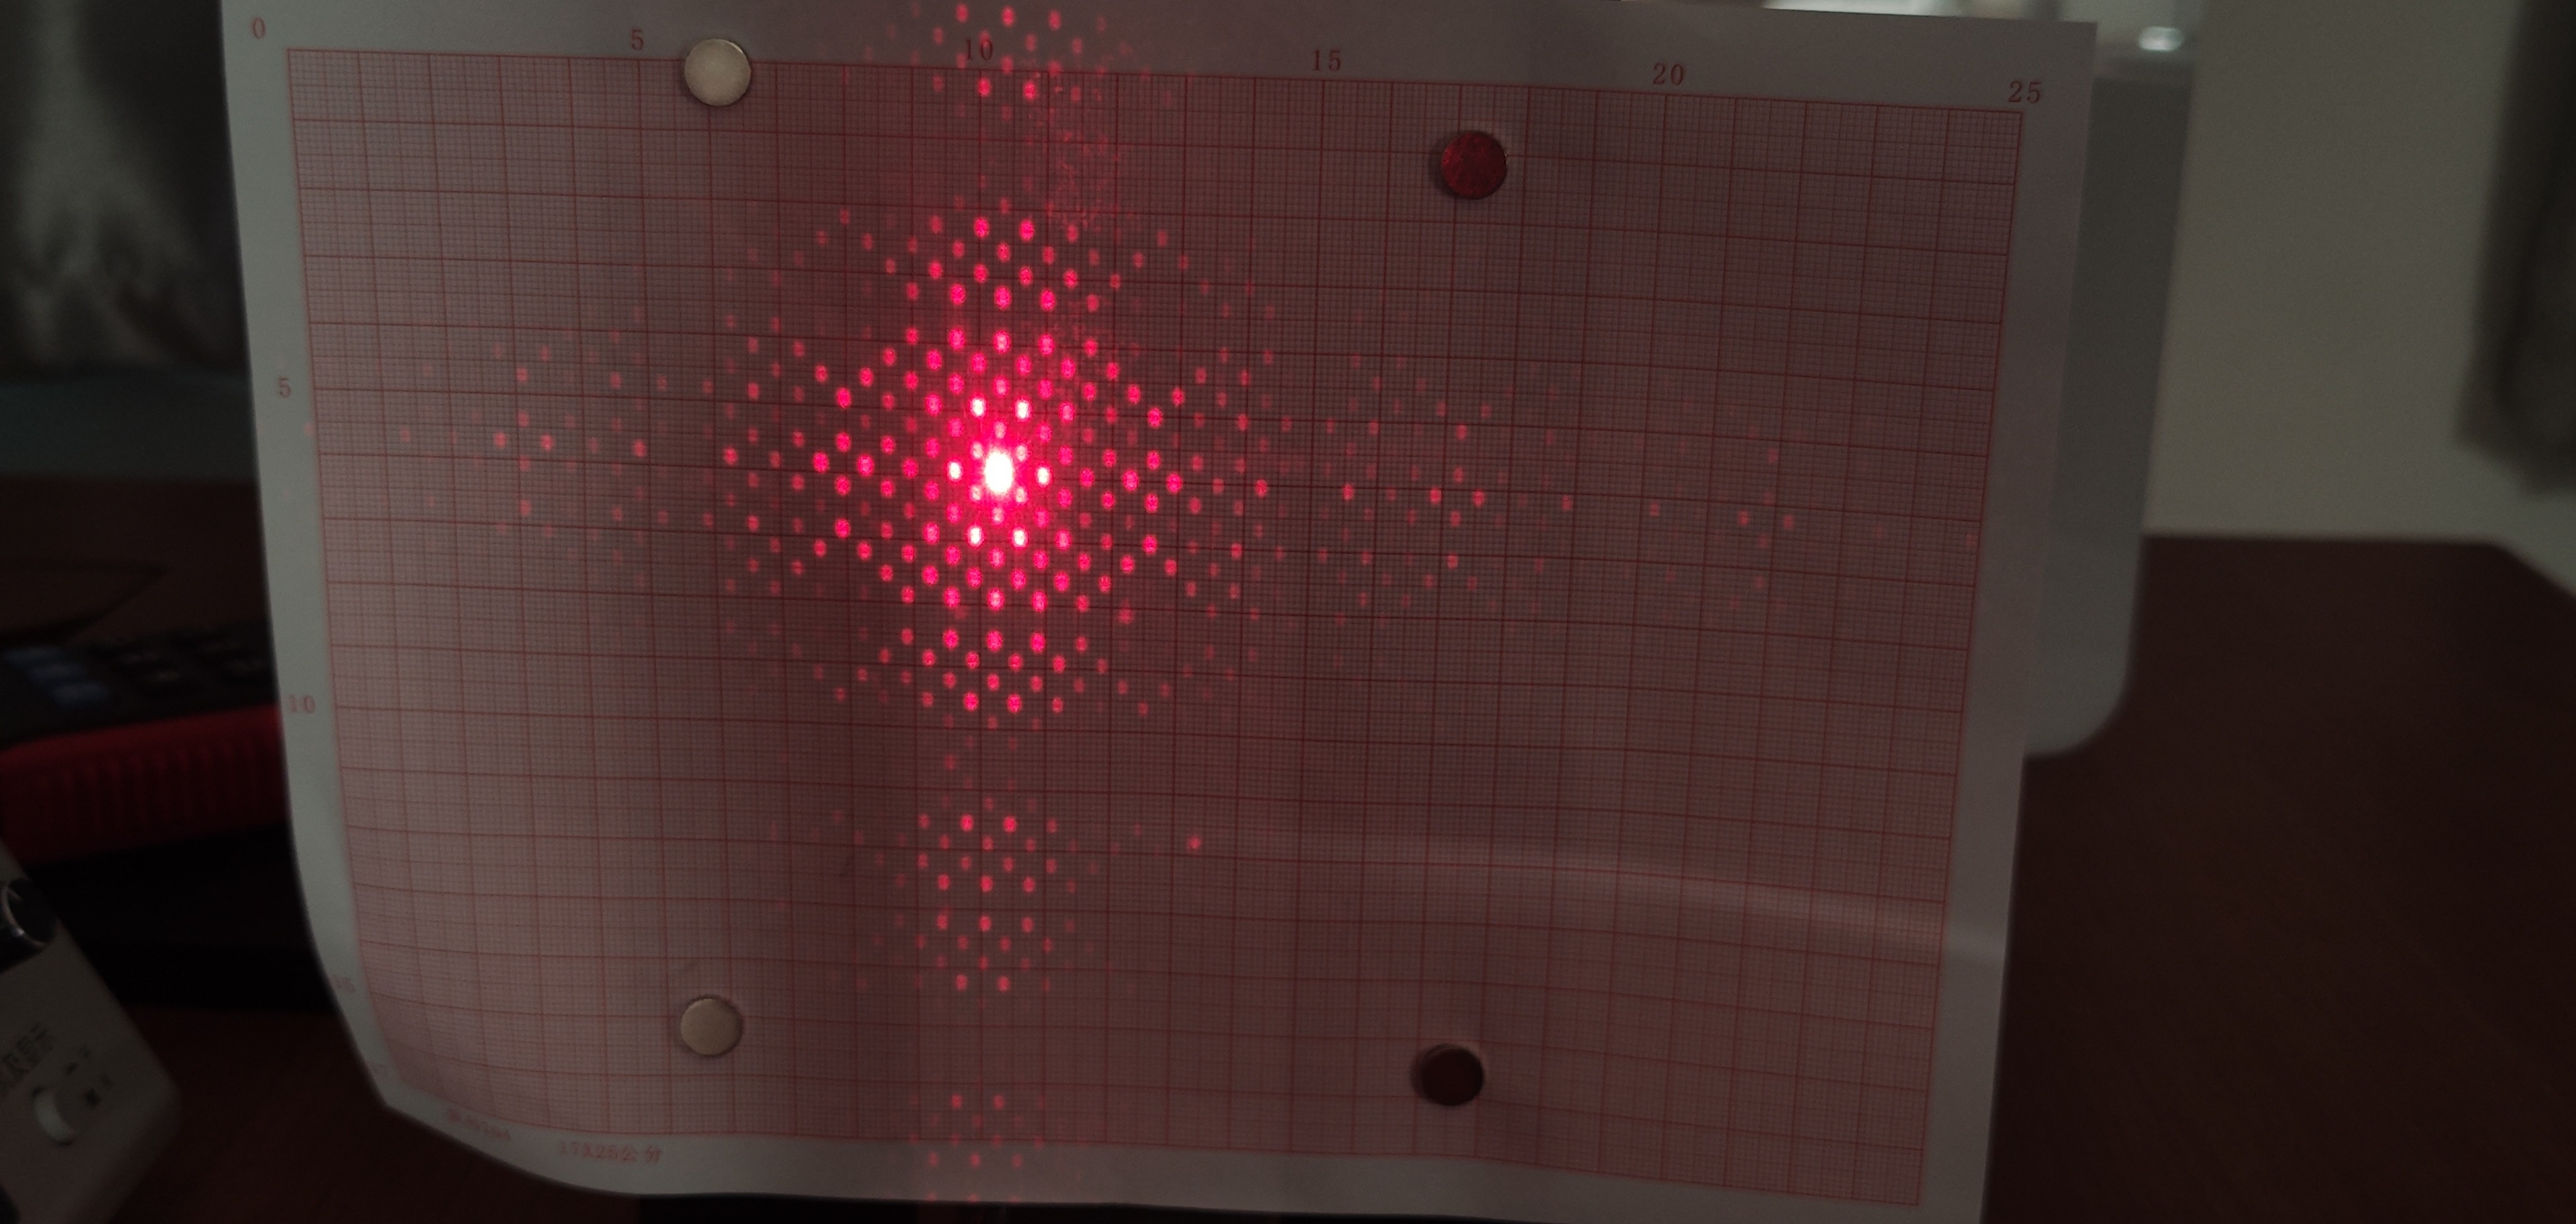
\includegraphics[width=\linewidth]{PG1.jpg}
	\caption{PG1}
	\label{fig:pg1}
\end{figure}
\begin{figure}[htbp]
\centering
	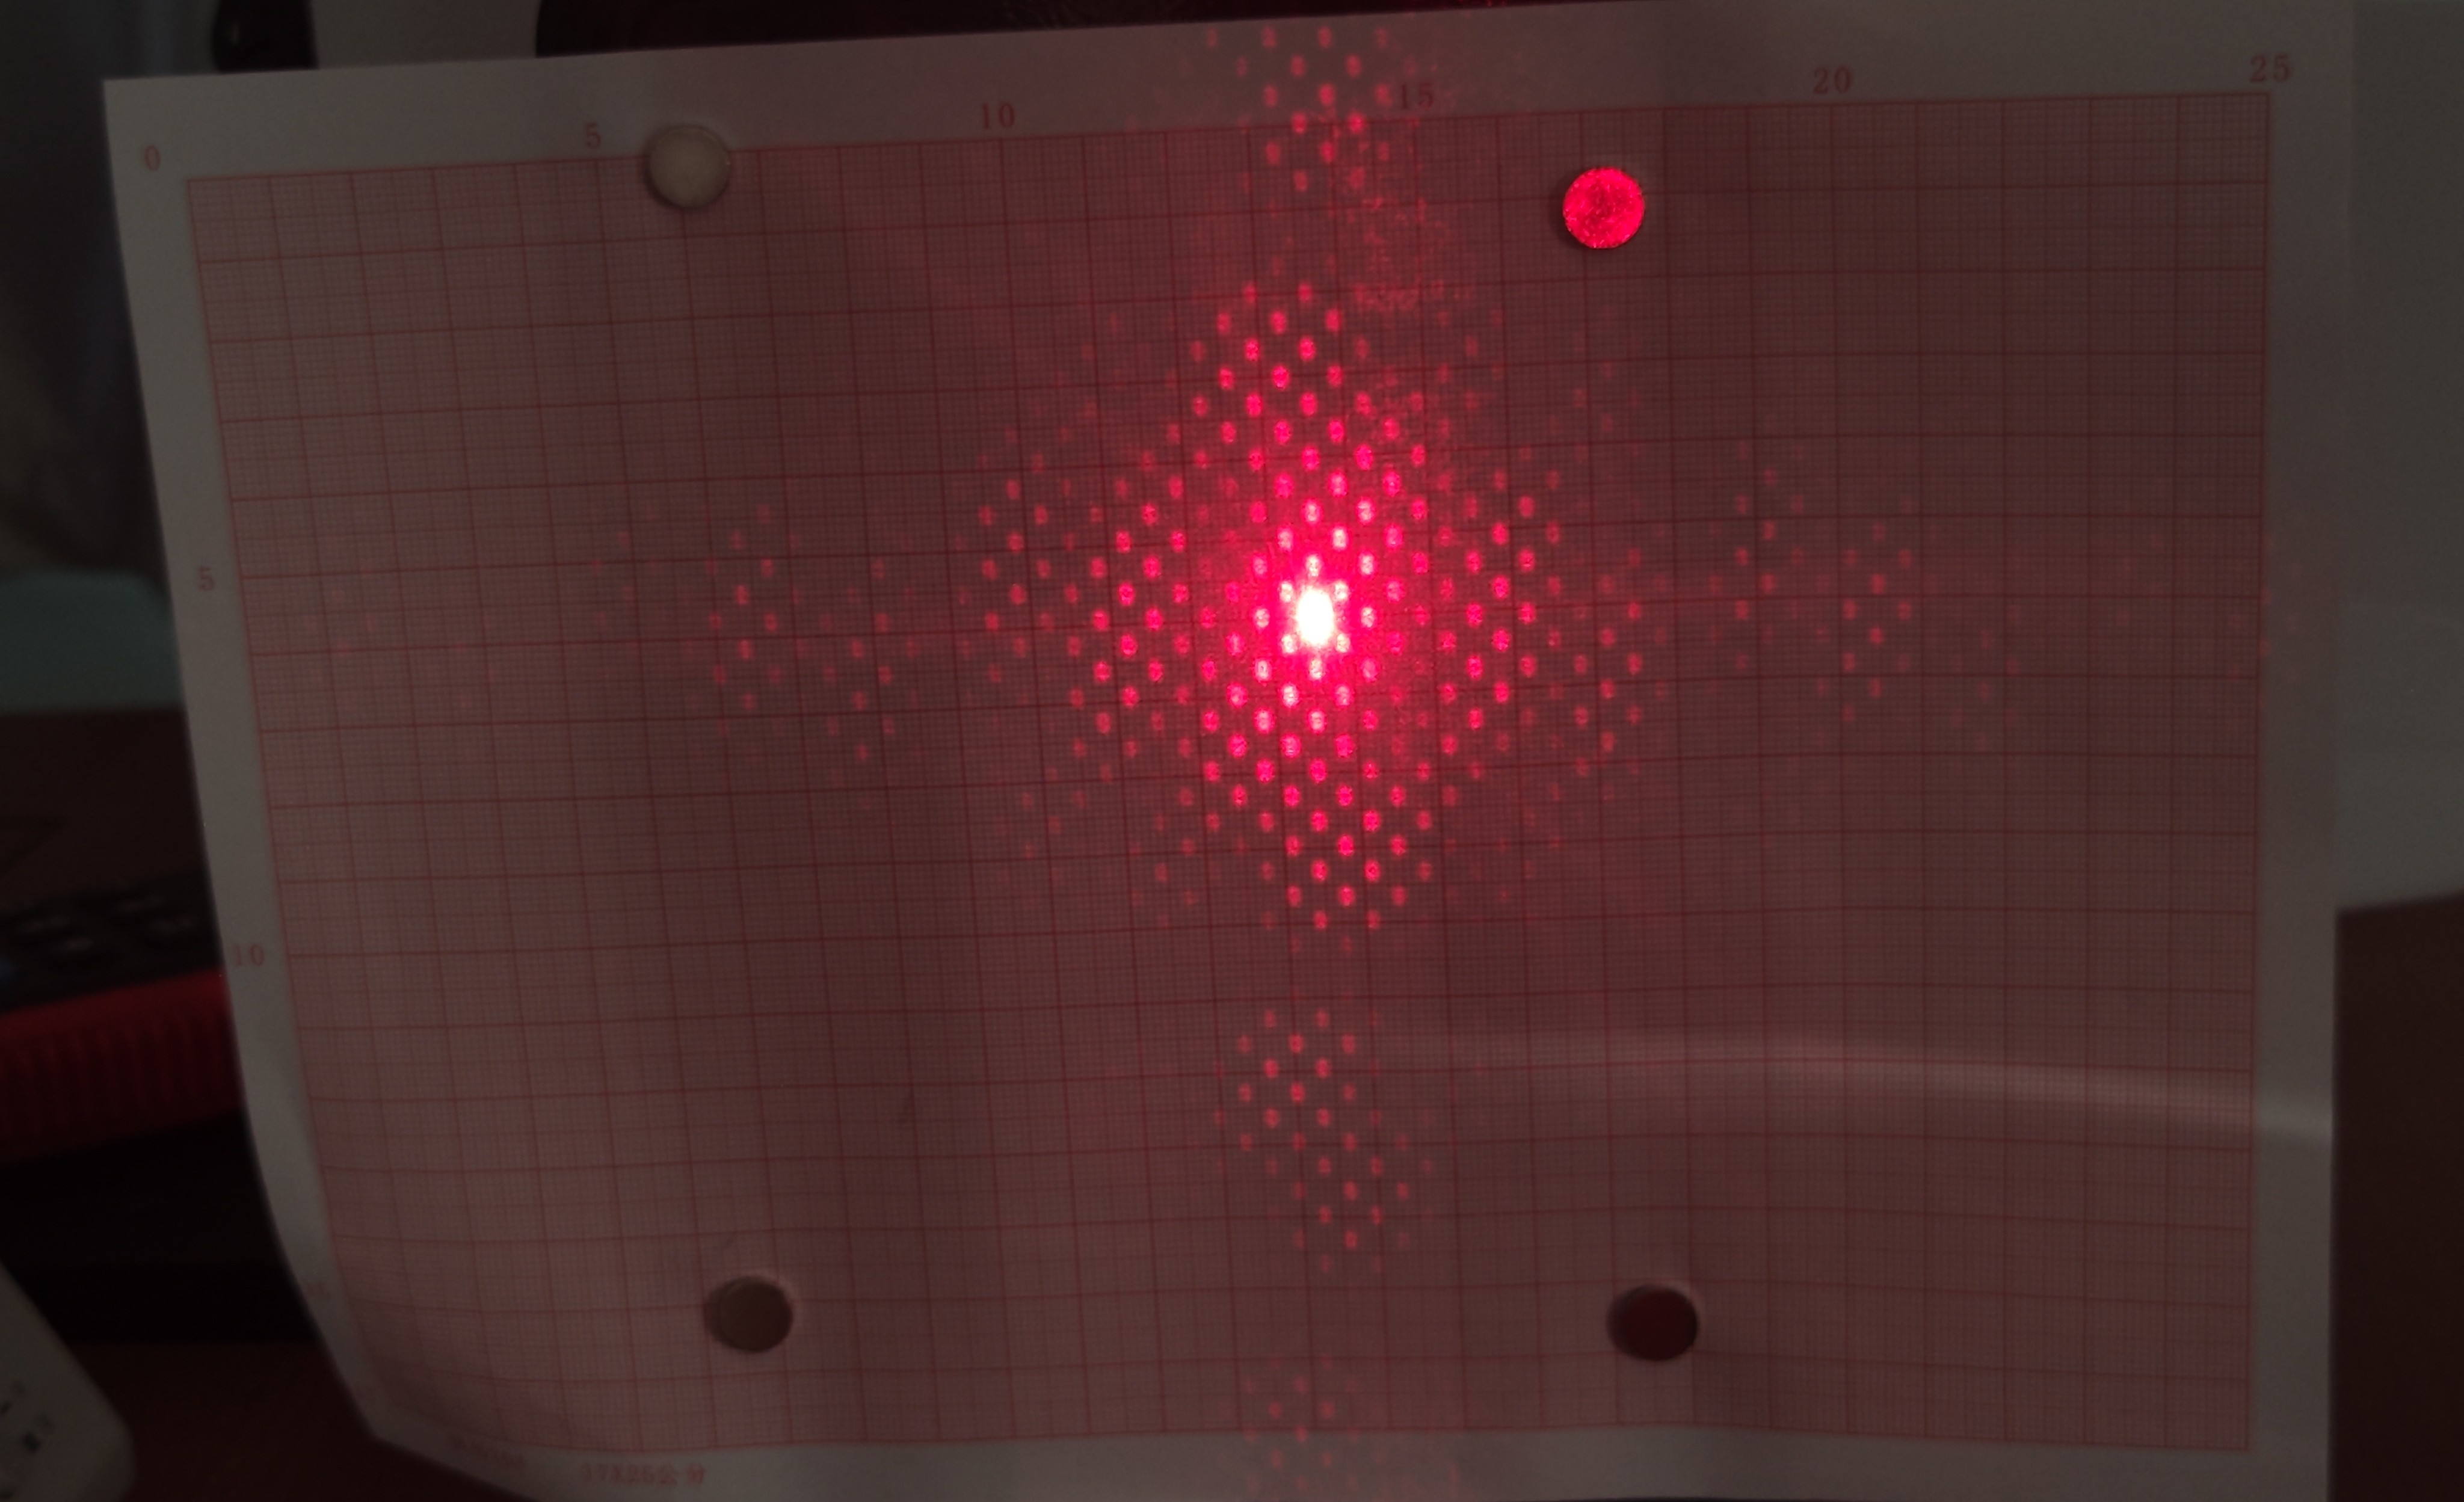
\includegraphics[width=\linewidth]{PG2.jpg}
	\caption{PG2}
	\label{fig:pg2}
\end{figure}
\begin{figure}[htbp]
\centering
	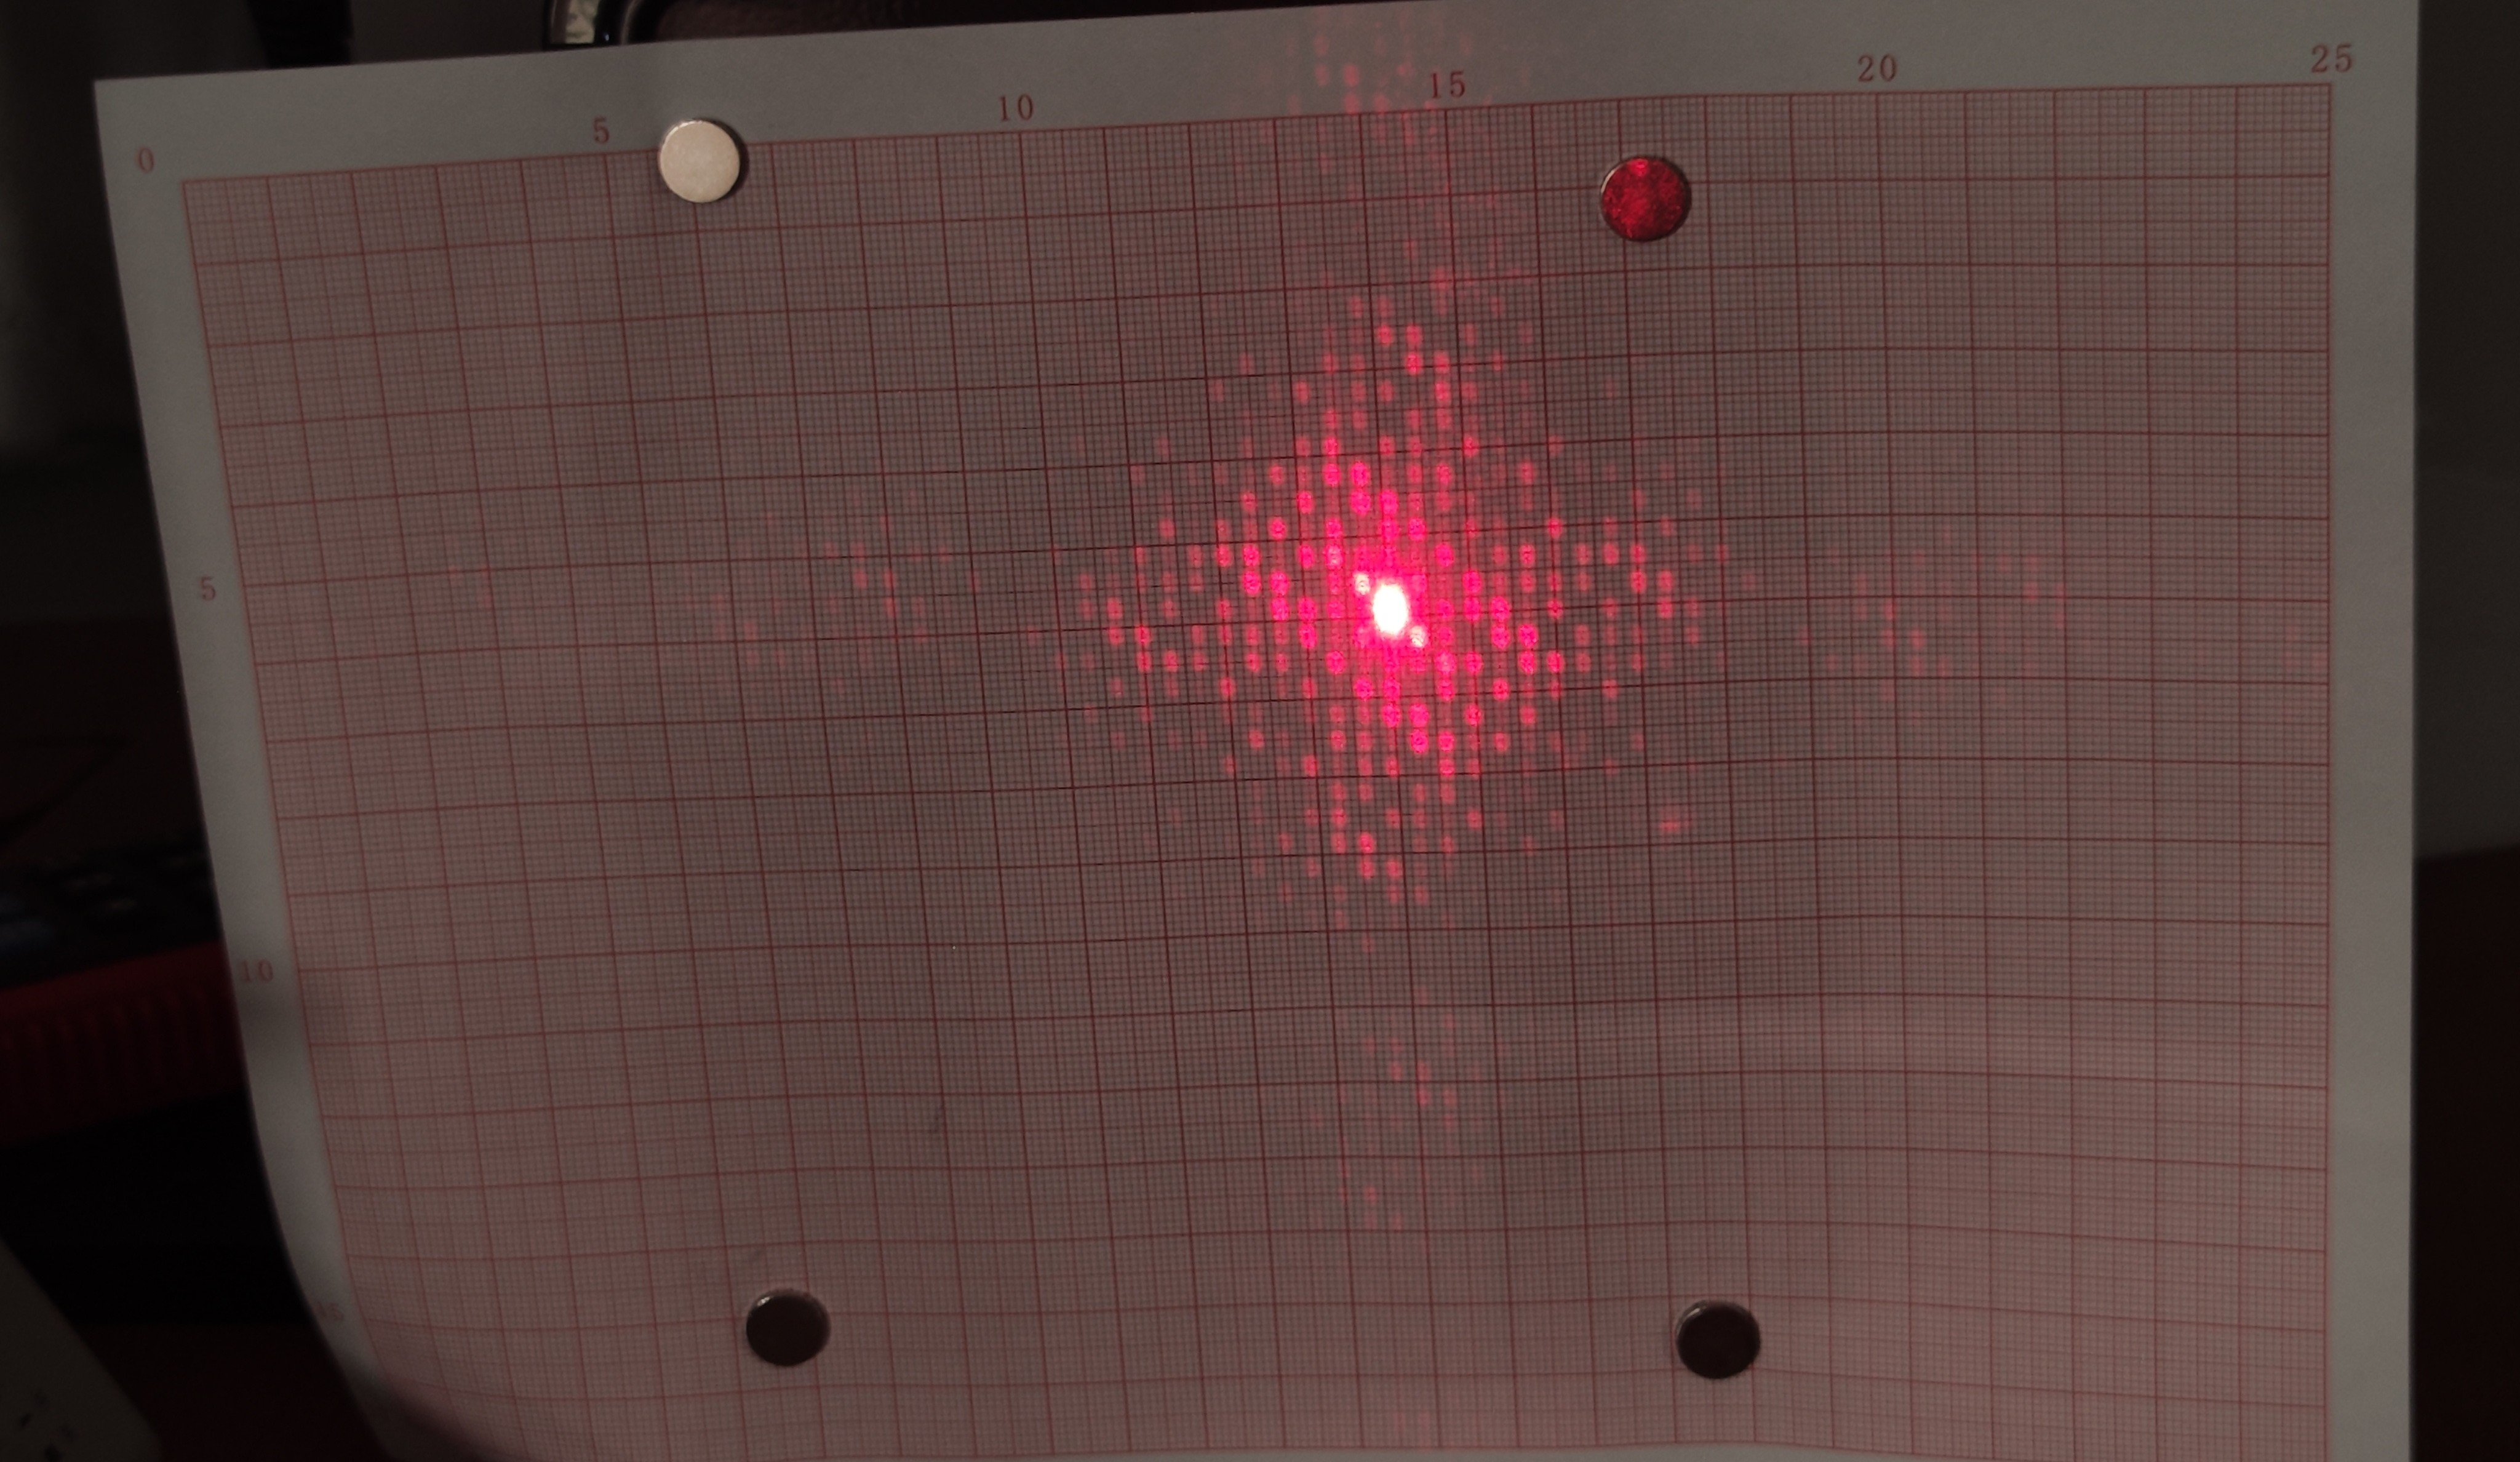
\includegraphics[width=\linewidth]{PG5.jpg}
	\caption{PG5}
	\label{fig:pg5}
\end{figure}
\begin{figure}[htbp]
\centering
	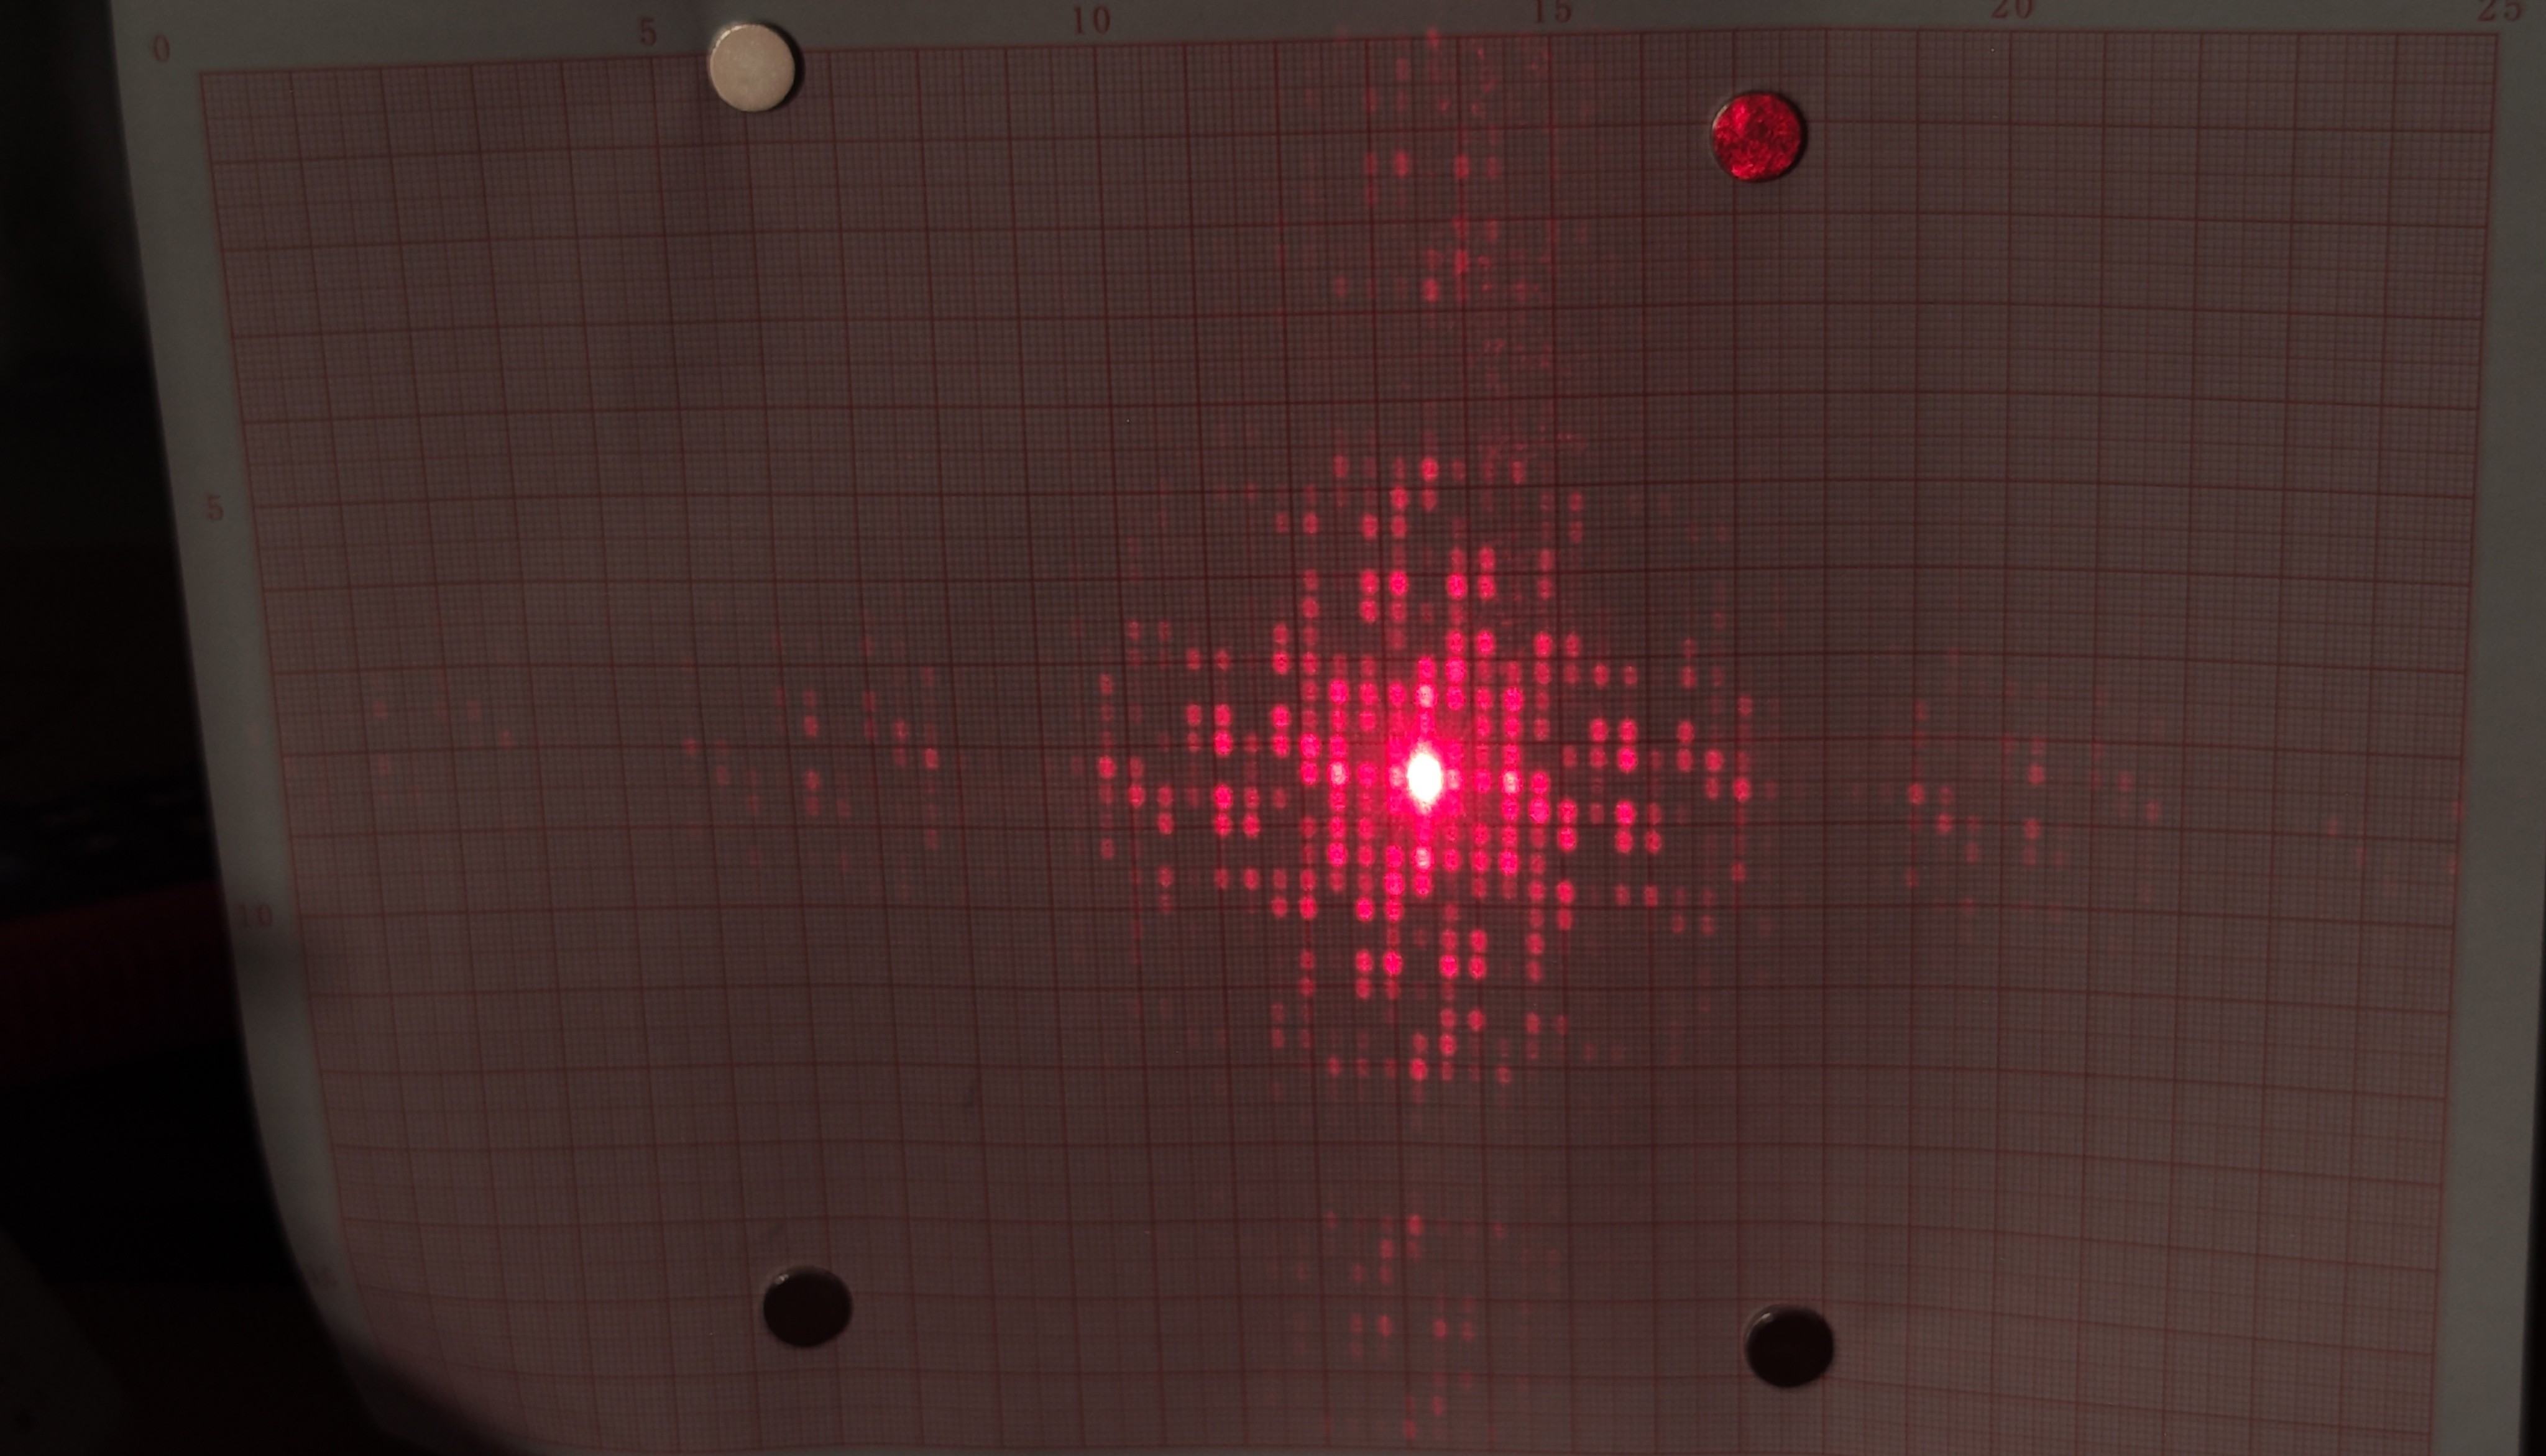
\includegraphics[width=\linewidth]{PG8.jpg}
	\caption{PG8}
	\label{fig:pg8}
\end{figure}
\begin{figure}[htbp]
\centering
	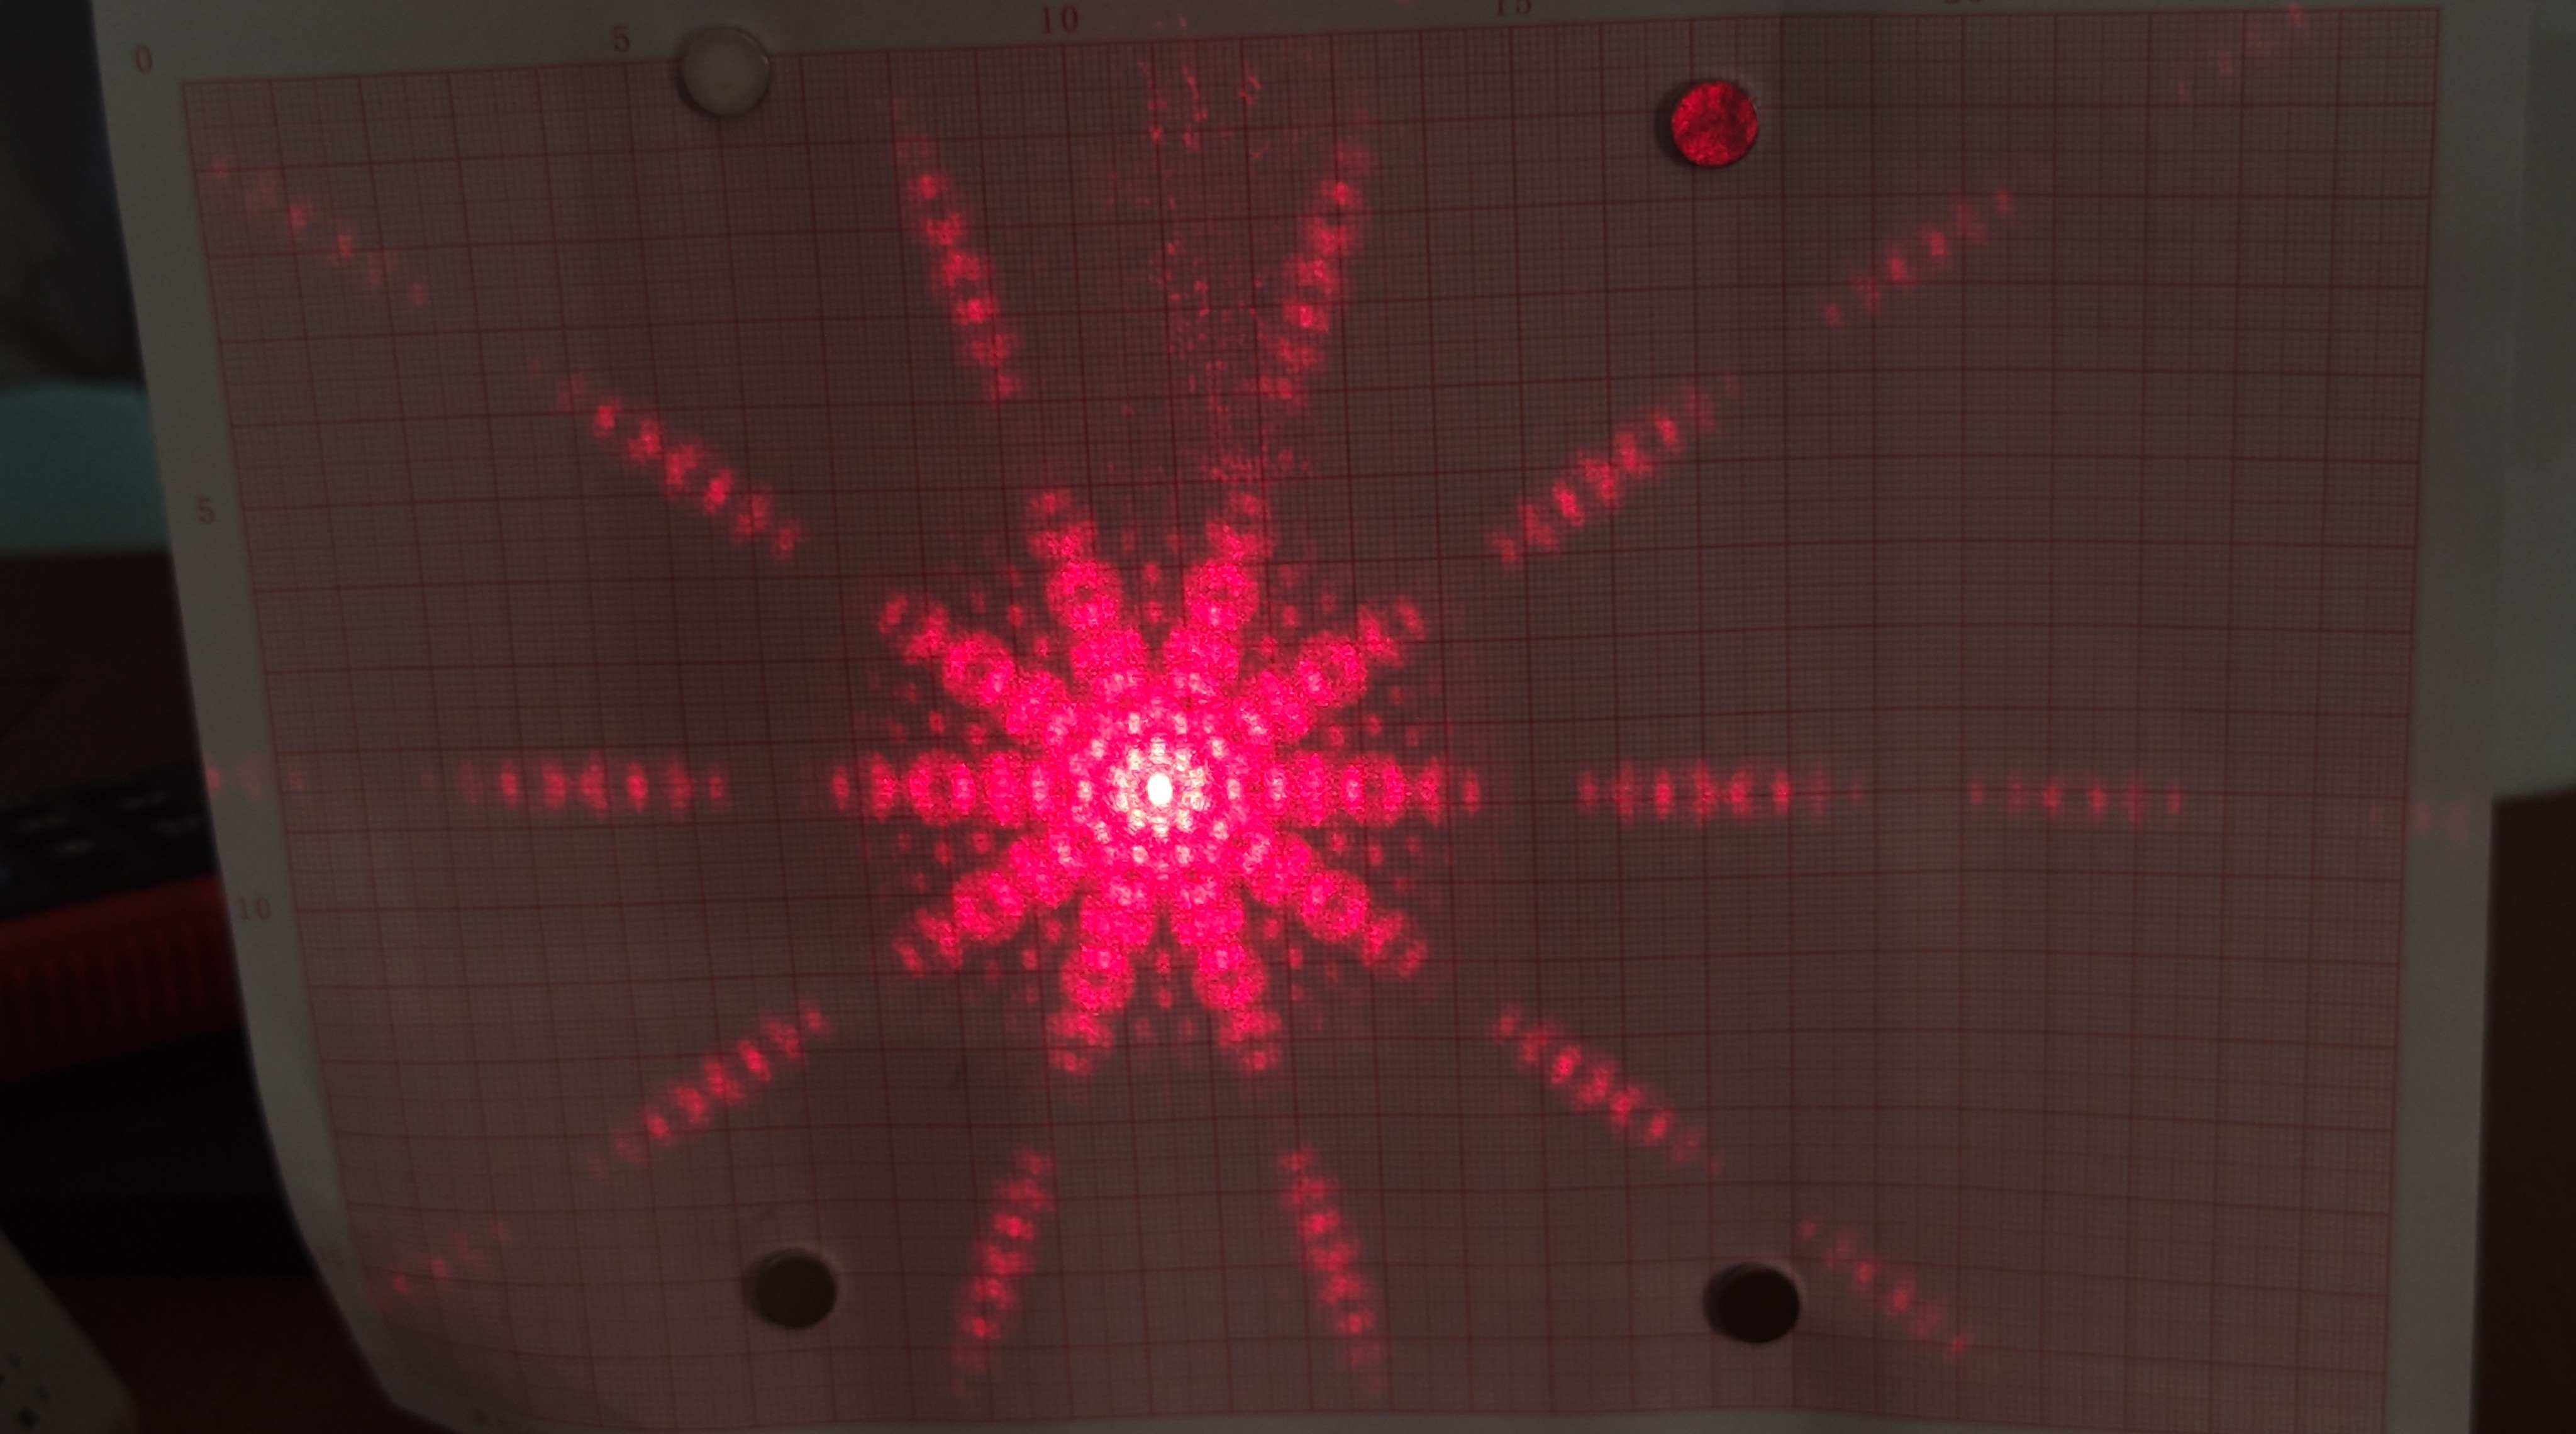
\includegraphics[width=\linewidth]{UC8.jpg}
	\caption{UC8}
	\label{fig:uc8}
\end{figure}

\section{由针对衍射强度的测量计算晶体结构}

原理上,我们期望的是通过对于衍射光斑强度做傅里叶变换来得到晶格各处的透射率,当然,这里是离散的情况,傅里叶变换变为一个双重求和。假设$\chi$和$\gamma$分别为晶格结构的水平和竖直坐标,在离散的情况下,有:
\begin{equation*}
	\begin{aligned}
		&\rho(\chi,\gamma) \\ 
		=&\sum_h\sum_k\sqrt{I}\cos{[\phi(h,k)-\frac{\pi}{2}(\chi h+\gamma k)]}
	\end{aligned}
\end{equation*}
根据这个原理,我们测量MR1的结构。麻烦在于,我们并不知道MR1的相位信息。这里可以采用以下措施补救:MR1与MR0的结构类似,激光通过二者应该有类似的相位信息,故可以采用MR0的相位来计算MR1。使用该方法,利用python编程计算,得到图\ref{fig:1}。由图可知,MR1具有晶胞结构X。
\begin{figure}[htbp]
\centering
	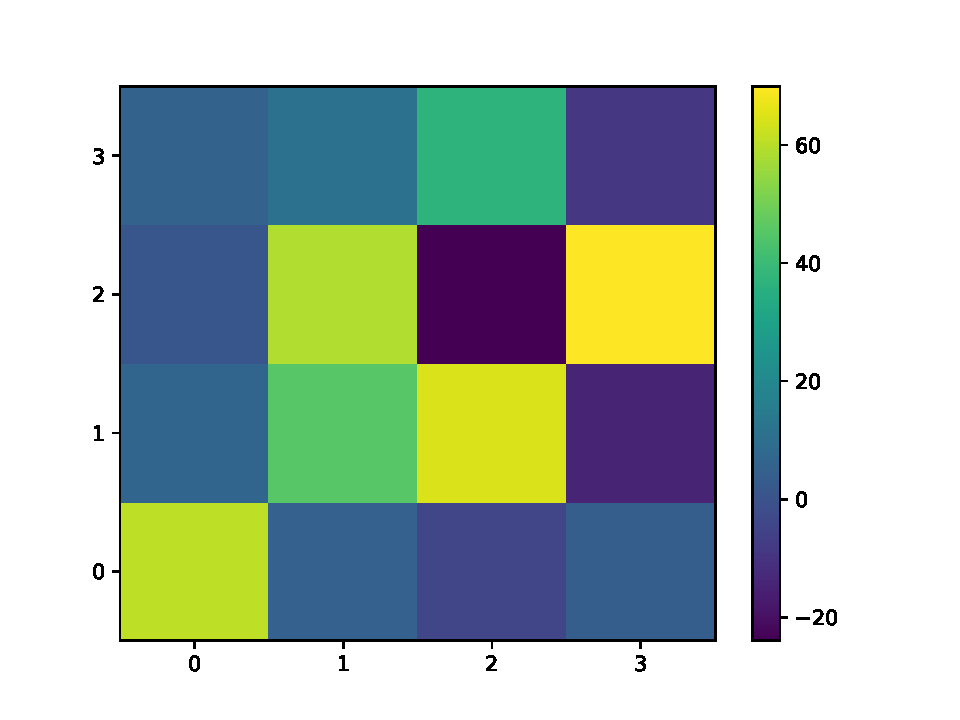
\includegraphics[width=\linewidth]{mr1.pdf}
	\caption{MR1的透射率}
	\label{fig:1}
\end{figure}
%------------------------------------------------



%----------------------------------------------------------------------------------------
%	APPENDIX
%----------------------------------------------------------------------------------------

%----------------------------------------------------------------------------------------

\end{document}
